\documentclass[11pt]{article}
\usepackage[margin=1in]{geometry}
\usepackage{amsmath,booktabs,graphicx,hyperref,caption}
\usepackage[round]{natbib}
\hypersetup{colorlinks=true,linkcolor=blue,citecolor=blue,urlcolor=blue}

% ---- post hoc illustration numbers (from data/logs/diag_F1_note.log and make_figures.py) ----
\newcommand{\MSharpeEUR}{17.8}
\newcommand{\MSharpeJPY}{16.0}
\newcommand{\MSharpeZN}{15.2}
\newcommand{\MWinRange}{91--98\%}

\title{News Timing Cannot Explain It:\\ A Pre-Registered Replication of Zhang (2025),\\
``Interpretable Machine Learning for Macro Alpha''}
\author{Timothy Oluwatobi Ojebiyi\thanks{Independent researcher. Email: \href{mailto:tobiojebiyi@gmail.com}{tobiojebiyi@gmail.com}.
Code, pre-registration, FinBERT scores and results: \url{https://github.com/coderback/zhang2025-replication}. I thank the GDELT Project and the authors of FinBERT for
public data and models. All errors are mine.}}
\date{October 2026}

\begin{document}
\maketitle

\begin{abstract}
\noindent
\citet{zhang2025} reports that FinBERT sentiment of GDELT news headlines, fed to an XGBoost classifier, predicts the
next-day direction of EUR/USD, USD/JPY and 10-year U.S.\ Treasury futures with cost-adjusted out-of-sample Sharpe
ratios of 5.87, 4.65 and 4.65 and daily win rates of 66--73\%. I rebuild the pipeline from the paper's description,
following its event filter, sentiment scoring, feature set, model classes, expanding-window validation and cost
assumptions on the paper's three assets, with headline text taken from article URLs rather than scraped pages. In a
pre-registered test, the XGBoost strategy earns Sharpe ratios of $-0.43$, $-0.05$ and $-0.73$, with win rates of
49--52\%, and none of the 18 asset $\times$ timing $\times$ model combinations earns a positive Sharpe ratio above
$0.02$. A variant that deliberately feeds the model the \emph{next} day's news also earns nothing, so misaligned news
timing cannot explain the reported performance; this rejects my own pre-registered hypothesis that it would. In a
post hoc illustration, a one-row shift in the lagged-return feature produces Sharpe ratios of 15--18, and applying
it to a random 39--48\% of days yields win rates and Sharpe ratios of the reported order. The reported results are
therefore unlikely to come from news sentiment. The findings agree with an independent replication by
\citet{andrews2026}, which tested EUR/USD, and extend it to the paper's other two assets and to a direct test of the
timing mechanism.
\end{abstract}

\noindent\textbf{Keywords:} replication, news sentiment, FinBERT, GDELT, foreign exchange, Treasury futures,
look-ahead bias, pre-registration.\\
\textbf{JEL:} C53, C58, F31, G14, G17.

\section{Introduction}
Out-of-sample return predictability is notoriously weak, for exchange rates \citep{meese1983} as for the equity
premium \citep{goyal2024}. A cost-adjusted Sharpe ratio near six from public news data would therefore be an
extraordinary result. \citet{zhang2025} reports exactly that. It combines the GDELT event database, the FinBERT
language model \citep{araci2019} and gradient-boosted trees \citep{chen2016}. The paper states that its code is
public, but the linked repository was not accessible when this note was written (September 2026). A first
independent replication \citep{andrews2026} found no predictive power. Its primary analysis kept all U.S.-related event
types across five assets, and a second, specification-matched analysis with the paper's CAMEO 100--199 filter found no
signal for EUR/USD (AUC 0.51, Sharpe ratio $0.10\pm0.91$ across folds). Two questions remain open:
\begin{itemize}
  \item the paper's other two assets, USD/JPY and 10-year Treasury futures, have not been tested with its filter;
  \item \citet{andrews2026} lists leakage and calculation errors, including the use of same-day market data, as
        plausible explanations, but no specific mechanism has been tested.
\end{itemize}

This note makes three contributions:
\begin{enumerate}
  \item It applies the original event filter and specification to all three of the paper's assets, including
        USD/JPY and ZN for the first time.
  \item The design, the timing variants and the verdict criteria were pre-registered before any sentiment score or
        model output was computed. Every result is compared with random-sign strategies at identical costs.
  \item Three timing variants isolate the role of news alignment and show that it cannot generate the reported
        numbers. A post hoc illustration shows that a simple one-line error in a price feature can.
\end{enumerate}

\section{The original study}
The original pipeline has five stages:
\begin{enumerate}
  \item \textbf{Events.} Take GDELT events from January 2015 to April 2025 with three-digit event codes 100--199,
        and keep the top 100 events per day by number of articles.
  \item \textbf{Sentiment.} Score each event's headline with ProsusAI/FinBERT, with polarity $s=P(\text{pos})-P(\text{neg})$.
  \item \textbf{Features.} Aggregate the daily mean, dispersion, volume, article impact and Goldstein statistics,
        with lags, moving averages and rolling windows, plus the lagged return and 20-day volatility.
  \item \textbf{Models.} Predict next-day direction with logistic regression and XGBoost under a 5-fold
        expanding-window \texttt{TimeSeriesSplit}.
  \item \textbf{Trading.} Go long if $\hat p>0.5$, otherwise short, with costs of 0.02\% (FX) and 0.05\% (ZN) per
        round trip.
\end{enumerate}
Table~\ref{tab:headline} reproduces the headline claims.

Five features of the paper should raise a reader's prior of an error:
\begin{itemize}
  \item daily win rates of 66--73\%, far above what published daily FX and bond predictors achieve;
  \item a leftover drafting note under the results table (``Numerical values in this table must accurately reflect
        results from the full backtest period ending April 2025'');
  \item the description of CAMEO codes 100--199 as ``consultations, statements, and diplomatic or economic
        engagements'', when in CAMEO they cover demands, disapproval, rejection, threats, protest, force posture,
        reduced relations, coercion, assault and fighting \citep{cameo};
  \item trade counts that differ by a factor of four between models on the same asset (215 versus 917 for
        USD/JPY);
  \item total returns that do not match the stated test period: at the reported CAGRs, the reported total returns
        imply about 10.2 years of compounding (9.5 for ZN XGBoost), whereas the out-of-sample period is stated as
        early 2017 to April 2025, about 8.3 years.
\end{itemize}

\section{Replication design}
\paragraph{Pre-registration.} The design, the three timing variants, the verdict rules and a hypothesis were
committed on 28~September 2026 (commit \texttt{260681b}, 13:16 BST) in the author's private research repository,
before any FinBERT score or model output existed. On local file timestamps, the first GDELT file was downloaded at
13:17, FinBERT scoring began at 18:09 and the first model results were produced at 19:53. The text is reproduced
unchanged in the public repository, and I will give reviewers read access to the original commit on request. The
pre-registered hypothesis was that the reported performance came from timing: the method as described would fail,
while a one-day look-ahead in the news (variant L below) would reproduce it. The data rejected the second half of
that hypothesis. Choices the paper leaves open are marked in the pre-registration and listed in
Appendix~\ref{tab:deviations}.

\paragraph{Events.} GDELT~1.0 daily event exports, 1~January 2015 to 2~October 2024 (3,561 of 3,563 files; two are
missing at source). Events are filtered to three-digit \texttt{EventBaseCode} 100--199, and the top 100 per news day
by \texttt{NumArticles} are kept, without de-duplication. That gives 365,026 events when days are keyed by event date
and 356,100 when keyed by date added.

\paragraph{Headlines.} The original scraped each event's page. For articles up to ten years old, link rot makes that
impractical and biased, so headline text is taken from the URL slug (the path segment with the most words, with ids
and extensions removed).
\begin{itemize}
  \item 93\% of top events yield a usable slug.
  \item On a random sample of 1,000 URLs, only 389 pages still return a title. On those, FinBERT scores of slug and
        title correlate 0.66 and agree in sign 84.8\% of the time.
  \item The daily index averages about 93 headlines, so its noise from slug text is far smaller than that of
        single headlines.
\end{itemize}
The 237,618 unique slugs are scored with ProsusAI/FinBERT (maximum 64 tokens, which covers slug-length text).

\paragraph{Features, targets and models.} Features follow Sections~3.3--3.4 of the original as specified. Prices are
Yahoo Finance closes for \texttt{EURUSD=X}, \texttt{USDJPY=X} and \texttt{ZN=F}, as in the original. The ZN series is
used as downloaded, without the roll adjustment the original describes. The target is
$y_t=\mathbb{1}[\log(P_{t+1}/P_t)>0]$. Both models are tuned by an inner \texttt{TimeSeriesSplit(3)} on each
training window only (the original uses five inner folds for XGBoost):
\begin{itemize}
  \item logistic regression, $C\in\{0.01,0.1,1,10\}$;
  \item XGBoost, depth $\in\{2,3,4\}$, learning rate $\in\{0.03,0.1\}$, $\lambda\in\{1,5\}$, up to 500 trees
        with early stopping on the last 20\% of the window.
\end{itemize}
The outer split is \texttt{TimeSeriesSplit(5)}, as in the original.

\paragraph{Timing variants.} The variants differ only in which news day feeds the prediction made at the close of
trading day $t$:
\begin{itemize}
  \item \textbf{P}: events dated $t$, the original as described;
  \item \textbf{S}: events added on the calendar day before $t$, so all news strictly predates the close;
  \item \textbf{L}: events dated on the next trading day $t{+}1$, the same day as the return being predicted. This is
        a deliberate look-ahead.
\end{itemize}
If the original's performance came from misaligned news, L should reproduce it.

\paragraph{Inference.} Out-of-sample daily returns are pooled across folds (from July or August 2016, depending on
asset and variant, to 30~September 2024). Significance is a one-sided block bootstrap with 21-day blocks. Each
strategy is also compared with 20 random-sign strategies on the same days at the same costs. The window ends in
September 2024, not April 2025, because later data is reserved as a hold-out in the wider research programme this
replication belongs to (Appendix~\ref{tab:deviations}). The pre-registered verdict rules use XGBoost under variant P;
the logistic results and the other variants are diagnostic.

\section{Results}
Table~\ref{tab:headline} compares the headline numbers, Table~\ref{tab:all} reports every combination, and
Figure~\ref{fig:cum} shows the growth of \$1 against the reported growth rates.
The outcome is the pre-registered ``not replicated, unexplained'' verdict: P is below a Sharpe ratio of 1 on every
asset, and L is below 2.
\begin{itemize}
  \item \textbf{The replication fails on every asset.} XGBoost under the original's own timing earns Sharpe ratios
        of $-0.43$ (EUR/USD), $-0.05$ (USD/JPY) and $-0.73$ (ZN), with win rates of 48.8--51.9\%.
  \item \textbf{Nothing is distinguishable from random trading.} Across all 18 combinations, Sharpe ratios lie
        between $-1.00$ and $+0.02$, and win rates between 47\% and 52\%. No XGBoost strategy exceeds the 95th
        percentile of its random-sign twins. The ZN twins are themselves negative because frequent sign changes at
        0.05\% per round trip are costly. The one strategy above its twins' 95th percentile, logistic ZN under
        variant L ($-0.48$ against $-0.67$), changes position on 43\% of days against the twins' 50\% and so pays
        less in costs. Before costs its Sharpe ratio ($+0.49$) is below the twins' 95th percentile ($+0.55$, 200
        draws), and after costs it still loses money.
  \item \textbf{The logistic baseline is also negative.} It has almost no tuning freedom, so the failure does not
        depend on the hyperparameter grid.
\end{itemize}

\begin{table}[t]\centering
\caption{Headline comparison: XGBoost, cost-adjusted, out of sample.}\label{tab:headline}
\begin{tabular}{lccc}\toprule
 & EUR/USD & USD/JPY & 10y Treasury (ZN)\\\midrule
Original: Sharpe (win rate) & 5.87 (72.7\%) & 4.65 (72.1\%) & 4.65 (66.1\%)\\
Replication P: Sharpe (win rate) & $-0.43$ (49.4\%) & $-0.05$ (51.9\%) & $-0.73$ (48.8\%)\\
Replication P: one-sided $p$ & 0.89 & 0.57 & 0.99\\\bottomrule
\end{tabular}
\end{table}

\begin{table}[t]\centering
\caption{All combinations. Sharpe ratios of the pooled out-of-sample daily returns, net of costs; $p$ is the
one-sided block bootstrap for XGBoost. ``Twins p95'' is the 95th percentile of 20 random-sign strategies on the same
days at identical costs.}
\label{tab:all}
\begin{tabular}{llrrrr}\toprule
Asset & Variant & Logistic & XGBoost & XGBoost $p$ & Twins p95\\\midrule
EUR/USD & P (as described) & $-0.09$ & $-0.43$ & 0.89 & 0.30\\
        & S (strict)       & $-0.06$ & $-0.66$ & 0.97 & 0.09\\
        & L (look-ahead)   & $-0.50$ & $-0.31$ & 0.84 & 0.30\\
USD/JPY & P & $-0.28$ & $-0.05$ & 0.57 & 0.31\\
        & S & $-0.51$ & $0.02$  & 0.48 & 0.15\\
        & L & $-0.43$ & $-0.29$ & 0.82 & 0.31\\
ZN      & P & $-0.77$ & $-0.73$ & 0.99 & $-0.67$\\
        & S & $-0.85$ & $-1.00$ & 0.997 & $-0.50$\\
        & L & $-0.48$ & $-0.71$ & 0.98 & $-0.67$\\\bottomrule
\end{tabular}
\end{table}

\begin{figure}[t]\centering
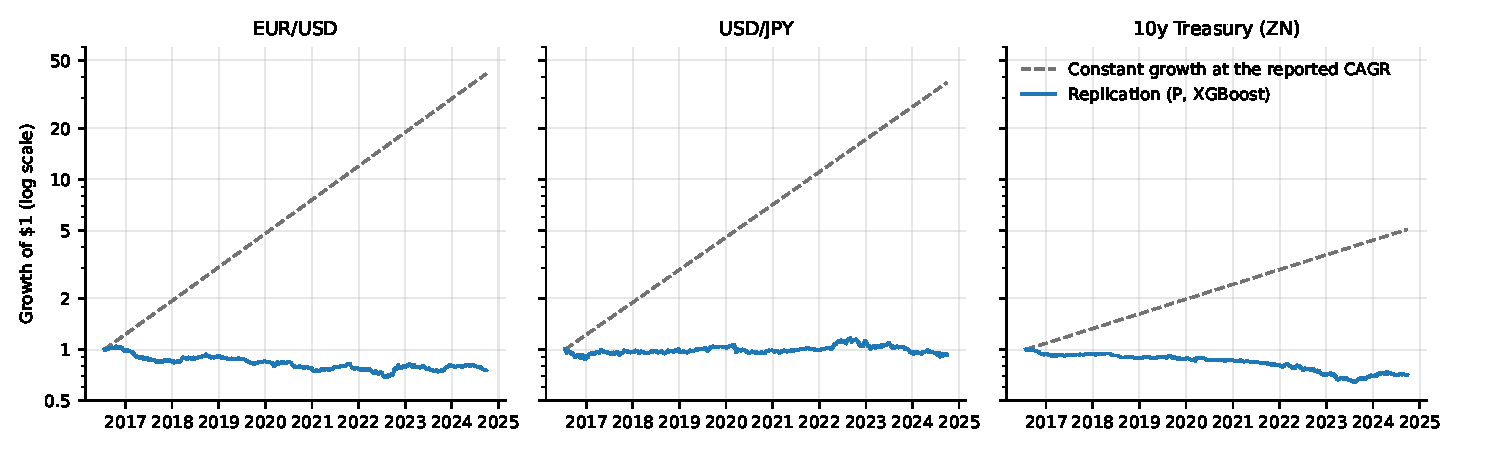
\includegraphics[width=\linewidth]{fig_cumulative.pdf}
\caption{Growth of \$1 for the replication's XGBoost strategy under the original timing (solid), out of sample, net
of costs. The dashed line is constant growth at the original's reported CAGR over the same dates, for scale; it is
not the original's equity curve.}\label{fig:cum}
\end{figure}

\section{What could produce the reported numbers?}
Figure~\ref{fig:sharpe} places every explanation on one axis. The three news-timing variants sit inside the range of
random trading, a fully shifted price feature overshoots the reported figures threefold, and a partial shift lands
on them.

\begin{figure}[t]\centering
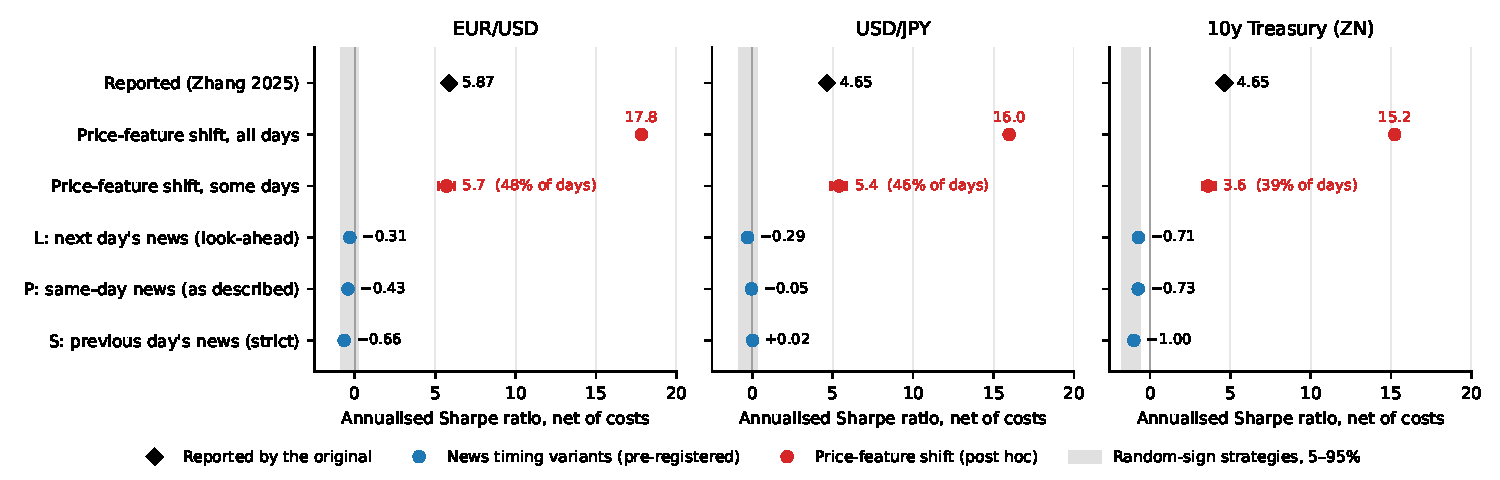
\includegraphics[width=\linewidth]{fig_sharpe.pdf}
\caption{Sharpe ratios by explanation, XGBoost, out of sample, net of costs. Blue: the pre-registered news timing
variants. Red: the post hoc price-feature shift, on all days or on a random share of days chosen to match the
reported win rate (mean and 5--95\% range over 200 draws). Gray band: 5--95\% range of 200 random-sign strategies
on the same days at the same costs; for ZN it lies below zero because frequent position changes are costly.}
\label{fig:sharpe}
\end{figure}

\paragraph{News timing cannot.} Variant L gives the model a full day of future headlines and still earns nothing.
Summarised as in the original, these headlines (top-coverage conflict and coercion events) carry no usable
information about next-day FX or Treasury moves. P, S and L cover news from before, on and after the prediction day,
and none comes close to the reported performance, so a misalignment of the news cannot explain it. The explanation
must lie elsewhere in the pipeline.

\paragraph{A price-feature shift can (post hoc illustration).} This analysis was designed after the results above
and was not pre-registered. The original feeds the model the lagged return $r_t$. If a one-row shift error made that
feature equal $r_{t+1}$, the return whose sign is the target, the pipeline would learn it directly. Re-running variant
P with this single change gives Sharpe ratios of \MSharpeEUR{} (EUR/USD), \MSharpeJPY{} (USD/JPY) and \MSharpeZN{}
(ZN), with win rates of \MWinRange{}. These exceed even the reported figures. A partial version of the error, such as
a date merge that misaligns only some rows, gives smaller numbers. I simulate this by letting each day independently
take the leaked position with probability $q$, choosing $q$ so that the expected win rate equals the reported one:
\begin{itemize}
  \item EUR/USD, $q=0.48$: win rate 72.0\%, Sharpe 5.7 (reported 72.7\% and 5.87);
  \item USD/JPY, $q=0.46$: win rate 72.8\%, Sharpe 5.4 (reported 72.1\% and 4.65);
  \item ZN, $q=0.39$: win rate 64.0\%, Sharpe 3.6 (reported 66.1\% and 4.65).
\end{itemize}
Win rates fall slightly short of the target because mixing positions adds trading costs. The reported win rates and
Sharpe ratios are thus jointly of the order that a partial leak produces. This is one concrete form of the
``same-day market data'' leakage that \citet{andrews2026} lists as a plausible source, and that study reports a
related experience: bugs in its own backtest initially produced Sharpe ratios of 11--16 at an AUC of 0.50. None of this is
evidence of what the original code did, which cannot be inspected. It shows how a one-line error of this kind
produces numbers of the reported order, whereas no treatment of the news timing does. Other candidates, including
leakage through hyperparameter selection or feature scaling fitted on the full sample, would need the original code
to assess.

\section{Robustness and limitations}
\begin{itemize}
  \item \textbf{Headlines} come from URL slugs, not scraped pages. The validation above suggests the daily index
        is a close proxy, and \citet{andrews2026}, who scraped headlines, also finds no signal.
  \item \textbf{The sample ends in September 2024} rather than April 2025. Even if the strategy had earned the
        reported Sharpe ratio in the missing seven months, the full-period Sharpe ratio would stay below 0.4 on every
        asset.
  \item \textbf{Other deviations} (GDELT~1.0 rather than the v2 API, three rather than five inner folds, a 64-token
        limit, an unadjusted ZN series) are listed in Appendix~\ref{tab:deviations}. None plausibly turns a Sharpe
        ratio near zero into one near five.
  \item \textbf{The hyperparameter grid} is mine, since the original gives none. The logistic model has almost no
        tuning freedom and is also negative.
  \item \textbf{The first out-of-sample day} is July or August 2016 rather than ``early 2017'', because
        \texttt{TimeSeriesSplit} divides the shorter sample differently. Restricting variant P to 2017 onwards
        (a post hoc check) gives Sharpe ratios of $-0.42$, $+0.11$ and $-0.62$. The USD/JPY sign changes, but all
        three stay near zero.
\end{itemize}

\section{Conclusion}
A pre-registered replication of \citet{zhang2025}, following the original's event filter, assets and methodology,
finds no predictive power: Sharpe ratios are near zero or negative everywhere, and win rates are at chance. Even
deliberately leaked future news cannot reproduce the reported performance, while a single shift in a price feature
can. Together with \citet{andrews2026}, the evidence indicates that the reported Sharpe ratios of 4.6--5.9 are
unlikely to arise from news sentiment as described. I contacted the author on 28~September 2026 to request the
code; any reply will be reflected in a revision.

\begin{thebibliography}{9}
\bibitem[Andrews(2026)]{andrews2026} Andrews, J.-P. (2026). A replication study of Zhang (2025): Why news sentiment
fails to predict asset returns. SSRN Working Paper 6426038. Code: \url{https://github.com/jandrews65/zhang2025}.
\bibitem[Araci(2019)]{araci2019} Araci, D. (2019). FinBERT: Financial sentiment analysis with pre-trained language
models. arXiv:1908.10063.
\bibitem[Chen and Guestrin(2016)]{chen2016} Chen, T., \& Guestrin, C. (2016). XGBoost: A scalable tree boosting
system. \emph{Proceedings of the 22nd ACM SIGKDD International Conference on Knowledge Discovery and Data Mining},
785--794.
\bibitem[Gerner et~al.(2002)]{cameo} Gerner, D. J., Schrodt, P. A., Y{\i}lmaz, \"O., \& Abu-Jabr, R. (2002).
Conflict and Mediation Event Observations (CAMEO): A new event data framework for the analysis of foreign policy
interactions. Paper presented at the Annual Meeting of the International Studies Association, New Orleans.
\bibitem[Goyal et~al.(2024)]{goyal2024} Goyal, A., Welch, I., \& Zafirov, A. (2024). A comprehensive 2022 look at
the empirical performance of equity premium prediction. \emph{Review of Financial Studies}, 37(11), 3490--3557.
\bibitem[Meese and Rogoff(1983)]{meese1983} Meese, R. A., \& Rogoff, K. (1983). Empirical exchange rate models of the
seventies: Do they fit out of sample? \emph{Journal of International Economics}, 14(1--2), 3--24.
\bibitem[Zhang(2025)]{zhang2025} Zhang, Y. (2025). Interpretable machine learning for macro alpha: A news sentiment
case study. arXiv:2505.16136v1.
\end{thebibliography}

\appendix
\section{Deviations from the original}\label{tab:deviations}
\begin{tabular}{p{0.28\linewidth}p{0.32\linewidth}p{0.32\linewidth}}\toprule
Item & Original & This replication\\\midrule
GDELT source & ``GDELT v2 API'', all events & GDELT 1.0 daily exports (same event fields)\\
Headline text & Scraped page titles & URL slugs (validated: corr.\ 0.66)\\
FinBERT input & Up to 512 tokens & Up to 64 tokens (slugs are short)\\
ZN prices & \texttt{ZN=F}, roll-adjusted & \texttt{ZN=F} as downloaded\\
Sample end & April 2025 & September 2024\\
Hyperparameters & ``Grid search'' (unspecified), five inner folds & Stated grid, three inner folds\\
Timing & One alignment & Three pre-registered variants (P, S, L)\\
Inference & Bootstrap CIs (not reported) & Block-bootstrap $p$ and random-sign twins\\\bottomrule
\end{tabular}

\end{document}
